%************************************************
\chapter{Basics of von Neumann algebras}\label{ch:von Neumann}
\minitoc\mtcskip
%************************************************

\noindent The following sections provide an elementary
introduction to the basic ingredients we shall be dealing 
with, namely operators on Hilbert spaces and von Neumann
algebras (\cite*{Jones:vN}). This is because the main features 
of a physical theory are encoded into the fields content, 
which in turn happen to emerge as operator valued distributions 
assigned to each point of the space-time, $x\mapsto\phi(x)$ 
(\cite*{Haag}). For this reason a systematic analysis of 
their mathematical properties is needed, and tools ought to 
be developed in order to better understand their algebraic 
underlying structure.


%*******************************************************
\section{Basic definitions and operator topologies}
\label{Operator topologies}
Let $\hil$ be a Hilbert space and $\dom{A}\subset\hil$.
An operator on $\hil$ whose domain is $\dom{A}$ is 
a linear map $A\colon\dom{A}\to\hil$.

 \begin{definition}[Operator norm]
 Let $x\in\dom{A}\mid x\neq 0$ and $A\colon x\mapsto A(x)\in\hil$.
 The operator norm of $A$ is defined as
 \begin{equation}
 \label{oper_norm}
 \norm{A}=\sup_{x\in\dom{A}\neq 0}\ 
 \frac{\norm{Ax}}{\norm{x}}.
 \end{equation}
 If $\norm{A}<\infty$ then the operator $A$ is said
 to be bounded.
 \end{definition}
 
 \begin{property}
 An operator $A$ is bounded if and only if it is continuous.
 \end{property}
 
 \begin{property}
 A bounded (and therefore continuous) operator $A$ defined
 on a dense subset $\dom{A}\subset\hil$ can be uniquely extended
 to the whole $\hil$ by continuity.
 \end{property}
 
As a remark we notice that, by continuity, the convergence of
the sequence $x_n\rightarrow x$ in $\dom{A}$ implies the 
convergence of the sequence $A x_n\rightarrow A x$. 

 \begin{definition}[Closed operator]
 Let $x_n\in\dom{A}$ such that $x_n\rightarrow x$. Let us also
 assume that $A x_n\rightarrow y$. The operator $A$ is called
 \emph{closed} if the previous assumptions imply $x\in\dom{A}$ and
 $y=A x$. Equivalently, an operator is closed if its graph is
 closed in the direct sum $\hil\oplus\hil$.
 \end{definition}
 
Take now an operator $A$, not necessarily closed, and assume that
the closure of its graph in $\hil\oplus\hil$ happens to be the graph 
of some operator $\overline{A}$, i.e. if $\overline{G(A)}=G(\overline{A})$.
Then $A$ is said to be ``closable'' and $\overline{A}$ its closure.

 \begin{definition}[Adjoint operator]
 Let $F_x\colon y\in\dom{A}\to\scal{x,Ay}\in\C$ for any operator
 $A$. The set of all points $\set{x\in\hil\mid F_x\text{ is continuous}}$ 
 is defined as $\dom{A^*}$. On this domain, by means of Riesz 
 representation theorem, $\exists !\,z\in\hil\mid F_x(y)=\scal{z,y}$.
 The operator $A^*$ adjoint of $A$ is defined as $A^*x=z$ on $\dom{A^*}$.
 \end{definition}
 
Given any two operators $A$ and $B$ we say that $A\subset B$ if
$\dom{A}\subset\dom{B}$ and $Ax=Bx$ on their common domain, i. e.
$x\in\dom{A}$. A densely defined operator is called \emph{symmetric} 
if $A\subset A^*$ and \emph{self-adjoint} if $A=~A^*$.

\bigskip
Henceforth let $\bh$ denote the set of all bounded operators
on a Hilbert space $\hil$, whose domains then coincide with the 
whole space, that is $\mathfrak{D}=\hil$. We assign the following topologies
on $\bh$ (\cite*{Jones:vN}):
 \begin{definition}[Topologies on $\bh$]
 Let $T_n$ be a sequence of operators and $T$ a ``limit point''
 in $\bh$: 
  \begin{enumerate}
  \item \emph{Norm topology}: $T_n\rightarrow T$ in norm if 
        $\norm{T_n-T}\rightarrow 0$ in the norm topology
        defined above in $\eqref{oper_norm}$.  
  \item \emph{Strong topology}: $T_n\rightarrow T$ strongly
        if $\forall\,x\in\hil$ then $\norm{T_n x- Tx}\rightarrow 0$ 
        in the vector norm of $\hil$.
  \item \emph{Weak topology}: $T_n\rightarrow T$ weakly if $\forall\,
        x,y \in \hil$ then $\scal{T_n x,y}\rightarrow\scal{Tx,y}$
        as complex functionals, i.e. $F_{x,y}(T_n)\rightarrow F_{x,y}(T)$.
  \end{enumerate}
 \end{definition}
 
It is easy to verify that a natural order among these 
topologies exists, namely
\[
\text{ norm topology }\vartriangleright
\text{ strong topology }\vartriangleright
\text{ weak topology}
\]
meaning that if a sequence of operators $T_n$ converges
to $T$ in a topology on the left then it converges
to $T$ in a topology on the right. Stronger topologies
have more open sets than weaker ones, and therefore 
if a set is closed in a weak topology it is also closed
in all the stronger ones.

 \begin{definition}[von Neumann algebra]
 A von Neumann algebra is a subset $\vN\subset\bh$ which is 
 closed under the weak operator topology and contains the
 identity. Its commutant ${\vN}'$ is defined as the set 
 ${\vN}'\coloneqq \set{m'\in\bh\mid \comm{m',m}=0,\ m\in\vN}$
 (similarly for $({\vN}')'={\vN}''$ and so forth).
 \end{definition}
 
 \begin{property}[von Neumann bicommutant theorem]
 Let $\vN={\vN}^*$ be a self-adjoint subalgebra of $\bh$. 
 The following assumptions are equivalent:
  \begin{enumerate}
  \item $\vN={\vN}''$.
  \item $\vN$ is weakly closed.
  \item $\vN$ is strongly closed.
  \end{enumerate}
 \end{property}

%*******************************************************
\section{Classification of factors}
\label{Classification of factors}
 \begin{definition}[Factor]
 The centre of an algebra is the set of all elements
 within that algebra which commute with all the rest,
 that is $Z(\vN)=\vN'\cap\vN$.  
 A von Neumann algebra $\vN$ whose centre is trivial 
 is called a factor, i.e. $Z(\vN)=\C\bm{1}$.
 \end{definition}
 
 \begin{definition}[Projections]
 $p\in\bh$ is called a \emph{projection} if and only if
 $p^2=p=p^*$. Likewise $v\in\bh$ is a \emph{partial isometry}
 if $v^* v=p$ is a projection. Given two projections
 $p$ and $q$, we say they are equivalent ($p\approx q$) 
 if there is a partial  isometry $v$ such that $vv^*=p$
 and $v^* v=q$.
 \end{definition}
 
Given two projections $p,q$ we say that $p\leq q$ if and only
if their ranges are $p\hil\subseteq q\hil$. In addition, a projection
$p$ is said to be minimal if, $\forall\,q\leq p$, either
$q=0$ or $q=p$. Consider now any $q\neq p, q<p$; if there is a partial
isometry $v\in\vN$ such that $v v^*=p$ and $v^* v=q$ then the 
projection $p$ is said to be \emph{infinite} (otherwise $p$
is called \emph{finite}). In a nutshell, then, a finite projection
has no equivalent subprojections, whereas infinite projections
do. Consequently a von Neumann algebra is called infinite if its identity 
is infinite, otherwise it is finite.

\bigskip
 \begin{definition}[Murray-von Neumann classification of factors]
 Projections allow us to classify factors according
 to the following:
  \begin{enumerate}
  \item  A factor $\vN$ with a minimal projection is called a
         Type I factor.
  \item  A factor $\vN$ with no minimal projections but non-zero
         finite projections is called a Type II factor.
  \item  An infinite factor $\vN$ admitting a non-zero linear
         functional (trace) $\tr\colon \vN\to\C$ such that
         
         {\centering
         \begin{enumerate}
          \item $\tr(xy)=\tr(yx)\quad x,y\,\in\vN$,
          \item $\tr(x^* x)\geq 0$,
          \item $\tr$ is ultraweakly continuous,
         \end{enumerate}
         }
         is called a Type $\textrm{II}_1$ factor. The trace is said
         to be normalised if $\tr(\bm{1})=1$.
  \item  A factor of the form $\vN\otimes\bh$, with $\vN$
         Type $\textrm{II}_1$ and $\textrm{dim}\ \hil =\infty$
         is called a Type $\textrm{II}_{\infty}$ factor.
  \item  A factor $\vN$ with no minimal projections, no non-zero
         finite projections is called a Type III factor.
  \end{enumerate}
  \begin{table}[tb]
  \caption{Type of factors}
  \centering
   \begin{tabular}{cp{0.8\textwidth}}
   \toprule
   Type & ``working'' definition\\
   \midrule
   I & with minimal projection; also $\exists\,\hil\mid \vN \cong \bh$.\\[0.5ex]
   II & no minimal projection but non-zero finite projections.\\[0.5ex]
   $\textrm{II}_1$ & infinite factor with no minimal projections
                   and a trace $\tr\colon \vN\to\C$.\\[0.5ex]   
   $\textrm{II}_{\infty}$ & $\vN\otimes\bh,\ \vN$ Type $\textrm{II}_1$
                            and $\textrm{dim}\ \hil =\infty.$\\[0.5ex]                           
   III & the rest, i.e. no minimal projections, no non-zero finite projections.\\
   \bottomrule
   \end{tabular}
  \end{table} 
 \end{definition}

%*******************************************************
\section{Introduction to modular theory}
\label{Introduction to modular theory}
Let $\vN\subset\bh$ be a von Neumann algebra and
$\Omega\in\hil$ a cyclic and separating vector for $\vN$.
The anti-linear operator
\begin{equation}
\label{Tomita}
S_0\colon a\Omega\mapsto a^*\Omega,\quad a\,\in\vN
\end{equation}
is closable (\cite*{BR:1979}) and in general unbounded. 
However, let $S=\overline{S_0}$ be
its closure and $S=J{\Delta}^{1/2}$ the respective polar
decomposition. We call $\Delta$ the modular operator and 
$J$ the modular conjugation associated with the pair
$(\vN,\Omega)$. Via functional calculus the
strongly continuous unitary group 
\[
\Delta^{it}=\e^{it \ln\Delta},\quad t\in\R
\]
may be defined and its adjoint action
\begin{equation}
\label{modular group}
\sigma^t_{(\vN,\Omega)}(m)\coloneqq \Delta^{it}\,m\,\Delta^{-it},
\quad m\,\in\vN,\ t\,\in\R
\end{equation}
induces a one-parameter automorphisms group of $\vN$ called
the \emph{modular automorphisms group}. 
A fundamental result in this respect is the

 \begin{theorem}[Tomita-Takesaki (\cite*{BR:1979})]
 Under the previous assumptions the following statements hold:
 the operator $J=J^*$ is anti-unitary and
  \begin{gather}
  J\vN J={\vN}'\\
  \sigma^t_{(\vN,\Omega)}(\vN)=\vN,\quad \forall\,t\,\in\R.
  \end{gather}
 \end{theorem}
The algebra is sent into its commutant by the adjoint action of the
modular conjugation $J$ and the modular group acting of $\vN$
exhausts all the algebra itself. Since all these quantities
explicitly depend on the pair $(\vN,\Omega)$ we have different
realisations of the modular automorphism group according to this choice. 
The characterisation of its shape, according to the choices 
of $(\vN,\Omega)$ in some particular cases, is the main topic 
of the work at hand.

 \bigskip
 The trivial case, i.e. when the algebra is commutative, is very
 easy to handle; take $a,b\,\in\vN$ and look at 
 $\scal{S\,a\Omega,S\,b\Omega}$, with $S$ defined as \eqref{Tomita}:
 \begin{align*}
 \scal{S\,a\Omega,S\,b\Omega}&=\scal{a^*\Omega,b^*\Omega}\\
 &=\scal{\Omega, ab^*\Omega}\\
 \intertext{by commutativity it follows then}
 &=\scal{\Omega, b^*a\Omega}=\scal{b\Omega, a\Omega}\\
 &=\overline{\scal{a\Omega,b\Omega}}
 \end{align*}
 therefore $S$ is antiunitary and hence $\Delta=\abs{S}=\bm{1}$.
 This implies that the action of the modular group
 is trivial on each element of the algebra.


 
 \subsection{\acf{KMS} condition}
 \label{KMS}
 Let $\vN$ be a von Neumann algebra and $\varphi$ a faithful normal
 state on $\vN$. Let furthermore $\sigma_t$ be a weakly
 continuous one-parameter group of automorphisms of $\vN$. 
 Fixed $a,b\,\in\vN$ consider $F_{a,b}(t)\coloneqq
 \varphi(a\,\sigma_t(b))$ as a function in the variable $t\,\in\R$.
 The state $\varphi$ is said to satisfy the Kubo-Martin-Schwinger
 (\ac{KMS}) condition at inverse temperature $T=\beta^{-1},\,0<\beta
 <\infty$ if 
 \begin{enumerate}
  \item $F_{a,b}(t)$ can be analytically continued in 
        the strip $0< \im{t}<\beta$. It is continuous at 
        the boundaries $\im{t}=0,\beta$ and
  \item $F_{a,b}(t+i\beta)=\varphi(\sigma_t(b)a)$.
 \end{enumerate}
 Notice that if the algebra were commutative then every state would
 satisfy the \ac{KMS} condition at $\beta=0$, by commutativity. 
 If this only happens as a special feature of the state at hand then
 $\varphi$ is said to be \emph{tracial}, otherwise $\beta\neq 0$ 
 measures the deviation of $\varphi$ from being a trace. Next note
 that a state is \ac{KMS} with respect to $\sigma_t$ at 
 $T^{-1}=\beta\neq 0$  if and only if it is \ac{KMS} with respect 
 to $\sigma_{-\beta t}$ at $T=-1$; therefore
 by rescaling the group parameter one can always refer to state
 of temperature $-1$. Albeit we shall not discuss this issue
 any further, \ac{KMS} states characterise equilibrium states in
 quantum thermodynamics where the one-parameter group $\sigma_t$
 plays the role of a given time evolution; however, to whom it may
 concern, a full characterisation and a systematic study of
 \ac{KMS} states is provided in \cite*{BRII:19781}.

 \medskip
 The remarkable connection with modular theory is that a normal
 state happens to be a \ac{KMS} state with respect to its own modular 
 group (\cite*{Haag}); the converse is also true, namely the modular 
 group is the only one-parameter group of inner
 automorphisms satisfying the \ac{KMS} condition on the state where it
 comes from. This feature will be fully used in the following to
 characterise and investigate properties of the modular group
 related to different states and algebras.
 
 
 
 \subsection{Bisognano-Wichmann property}
 \label{BiWi}
 As a matter of example let us consider a very important result obtained 
 by Bisognano and Wichmann (\cite*{BiWi:1975}), and so far the only (up to
 geometric transformations) explicit characterisation of modular operators
 for space-time regions.
 
 \medskip
 Let $\wed_{R,L}\coloneqq \set{x\in {\vN}^4\mid x^1\gtrless
 \abs{x^0}}$ be the right (left) wedge region as a subset of the space-time
 $\vN^4$. There is exaclty a one-parameter subgroup of the Lorentz
 group preserving the wedge, namely mapping the wedge into itself:
 \begin{equation}
 \label{Lor_boost}
 \Lambda(t)= \begin{pmatrix}
             \cosh(t)& -\sinh(t) & 0 & 0\\
             -\sinh(t)&\cosh(t) & 0 & 0\\
             0 & 0 & 1 & 0\\
             0 & 0 & 0 &1             
             \end{pmatrix}.
 \end{equation}
 Let the local von Neumann algebra $\alg{\wed}$ be generated by 
 Wightmann fields $W(f)$ and let us choose as a cyclic and separating vector
 the vacuum $\Omega$ as \ac{GNS} of $\vac\left(W(f)\right)=\e^{-1/2{\norm{f}}^2}$. 
 The modular group associated to the pair $\left(\alg{\wed},\Omega\right)$
 coincides with the unitary representation of the subgroup preserving
 the wedge and the modular conjugation acts as reflection through the edge
 of the wedge, changing sign to both $x^0$ and $x^1$
 \begin{equation}
 \label{BiWi}
 \Delta^{it}=U(\Lambda_{\wed}(-2\pi t))\qquad
 J=U(r_{\wed}).
 \end{equation}
 However, since the vacuum is invariant under Poincar\'{e}
 transformations $g$, this result can be generalised to any
 region of the form $\wed'= g\wed $. Setting
 (\cite*{Longo:private})
 \[
 \Lambda_{{\wed}'}(t)=g\,\Lambda_{\wed}\,g^{-1}
 \qquad
 r_{{\wed}'}=g\,r_{\wed}\,g^{-1} 
 \]
 we obtain (\cite*{Guido:2011} and \cite*{GLW:1998})
 \[
 \Delta^{it}=U(\Lambda_{\wed'}(-2\pi t))\qquad
 J=U(r_{\wed'}).
 \]
 It can be shown (again \cite*{Guido:2011}) that the 
 Bisognano-Wichmann property also holds for conformally 
 covariant theories that split into tensor products of 
 two nets on a line, as described in \ref{Conformal nets}. 
 In fact, in two dimensions a wedge reduces to the cartesian 
 product of two half-lines $\R_+\times\R_-$. In the particular
 case where $\I=\R^+$ the modular group explicitly acts as dilations
 with a scaling factor of $\e^{-2\pi t}$
 \[
 \sigma_t\blank=\delta_{\lambda_t}\blank,
 \qquad \lambda_t=\e^{-2\pi t}
 \]
 The two-dimensional modular flow is then $\delta_{\lambda_t}
 \otimes\delta_{\lambda^{-1}_t}$. Intervals can be obtained 
 as conformal transformations of the real line and hence 
 in this case the modular group, corresponding to the 
 subgroup of the Lorentz transformations preserving the wedge, 
 is replaced by the subgroup of the M\"obius transformations 
 fixing each interval, either on the circle picture $\s$ or 
 on the real line.
 
 \begin{minipage}{.35\textwidth}
 \centering 
 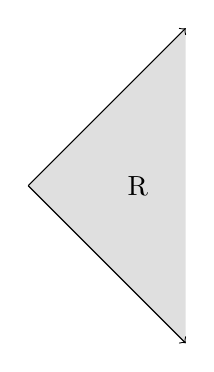
\begin{tikzpicture}[scale=2]
 \fill[gray!25] (0,0)--(1,1)--(1,-1);
 \draw [->] (0,0) -- (1,1);
 \draw [->] (0,0) -- (1,-1); 
 \node at (0.7,0) {$\wed_{\textrm{R}}$};
 \end{tikzpicture}
 \end{minipage}
 \qquad
 \begin{minipage}{.60\textwidth}
 \begin{tikzpicture}[scale=2]
 \draw [->] (0,0) -- (1,1);
 \node [rotate around={45:(-1.5,3)}] {\footnotesize $\R_+$};
 \node at (1.27,0.5) {$\bigtimes$};
 \draw [->] (1.5,1) -- (2.5,0);
 \node [rotate around={-45:(2.9,-5.8)}] {\footnotesize $\R_-$};
 \end{tikzpicture}
 \end{minipage} 
 
 \medskip
 As already mentioned above, the modular group $\sigma^t_{\Omega}$ 
 uniquely satisfies  the \ac{KMS} condition on $\Omega$ and hence
 it characterises thermal equilibrium states for an observer whose
 dynamics is given by $\sigma^t_{\Omega}$. According to this 
 interpretation, the Bisognano-Wichmann property for wedge regions 
 states that the vacuum state is a thermal equilibrium state with 
 temperature $T=-1$ for an observer accelerated with Lorentz boosts.
 This is the case for an observer moving around the event horizon
 of a black hole and the example provides an explanation of the
 Unruh effect, by which the vacuum state
 behaves like a thermal states for observers moving in a 
 gravitational field (\cite{ConRov:1994, MartRov:2003}). 
 In fact, the trajectory of an observer moving in such 
 an event horizon (corresponding in turn to a wedge region) 
 with constant acceleration $a$ is given by the orbits of the 
 Lorentz boosts of the form \eqref{Lor_boost} with the 
 proper ``physical'' time $\tau$ being $t/a$. 
 Therefore the trajectory in the wedge can be
 parametrised as 
 \[
 x^{\mu}(\tau)=1/a\,(\sinh(a\tau),\cosh(a\tau),0,0)
 \]
 and the evolution at later times is $x(\tau_0+\tau)=
 \Lambda(a\tau)x(\tau_0)$. On the other hand, as we 
 have seen in equation \eqref{BiWi}, the modular group 
 with respect to the vacuum state act as a Lorentz boost
 of parameter $-2\pi s$ and satisfies the \ac{KMS} 
 property. Therefore, by uniqueness, the relation between
 the physical time $\tau$ and the modular parameter $s$
 has to be $-2\pi s=a\tau$, in order to give back 
 the Unruh inverse temperature $\beta=-\dd \tau/\dd s=2\pi/a$.
 
 \subsection{Reconstruction of the translations}
 \label{Reconstruction of the translations}
 As just stated, the modular group associated with the pair
 $(\alg{\mathcal{W}},\Omega)$, $\mathcal{W}$ being a wedge region,
 acts like the associated group of Lorentz boosts and this 
 preserves the wedge itself. Remarkable results by Borchers 
 \cite*{Borch:1992} and Wiesbrock \cite*{Wies1,Wies2,Wies3}
 showed that it is possible, under suitable conditions, to
 recover the translations group out of modular data.
 
 \begin{definition}
 Let $\vN$ be a von Neumann algebra with a cyclic and separating
 vector $\Omega$. Let furthermore $U(a)\coloneqq \e^{iaH},\,a\in\R$, 
 be a continuous one-parameter group of unitaries with positive
 generator $H$ leaving $\Omega$ invariant, i. e. $U(a)\Omega=
 \Omega$. The triple $(\vN, H\geq 0, \Omega)$ is called a 
 ``Borchers triple''. Also, the triple is said to satisfy the 
 \emph{half-sided translations} condition if
 $\ad{U(a)}\vN\subset\vN,\ a>0$. 
 \end{definition}
 \begin{theorem}[\cite*{Borch:1992}]
 \label{Borchers}
 Let $\vN$ be a von Neumann algebra with a cyclic and separating
 vector $\Omega$ and denote as $\Delta, J$ the modular data of the pair
 $(\vN,\Omega)$. Then, given a half-sided translated Borchers 
 triple as above, the following  holds
 \begin{align}
 \Delta^{it}U(a)\Delta^{-it}&=U(\e^{-2\pi t}a)\label{Bor}\\
 JU(a)J&=U(-a), 
 \end{align}
 namely $U(a)$ is seen to satisfy translations-dilations commutation relations
 with~$\Delta^{it}$.
 \end{theorem}
 A stronger result provided by Wiesbrock holds true: given two algebras
 in suitable position one can automatically recover the unitaries
 $U(a)$ out of their modular operators only; the construction is showed
 below.
 \begin{definition}
 Let $\mathcal{N}\subset\vN$ be two von Neumann algebras with common
 cyclic and separating vector $\Omega$ and denote with $\Delta_{\vN},
 \Delta_{\mathcal{N}}$ the respective modular operators. We call the 
 inclusion $\mathcal{N}\subset\vN$ half-sided modular (\cite*{Wies1})
 if $\Delta_{\vN}^{-it}\mathcal{N}\Delta_{\vN}^{it}\subset\mathcal{N}$
 for $t\geq 0$.
 \end{definition}
 \begin{theorem}[\cite*{Wies1}]
 \label{Wies:th}
 Under the previous assumptions of half-sided modular inclusion
 $\mathcal{N}\subset\vN$ let $H\coloneqq 1/2\pi 
 \left(\ln \Delta_{\mathcal{N}}-\ln \Delta_{\vN}\right)$; 
 the triple $(\vN, H\geq 0, \Omega)$ is a half-sided translated
 Borchers triple fulfilling theorem \ref{Borchers}. 
 \end{theorem}
 This result suggests that the information about the translations
 is contained into the mutual positions of the two algebras and their
 common cyclic and separating vector. As an important application
 of such result we mention that wedge regions and their translated
 indeed satisfy the half-side modular inclusions and therefore
 the above results directly apply. Representations of the 
 Lorentz boosts emerge as modular operator $\Delta^{it}_{\vN}$ (as a 
 consequence of the Bisognano-Wichmann property) and  
 translations may be recovered by means of the Wiesbrock procedure
 (in two dimensions these exhaust the whole Poincar\'{e} group).
 

 

 
 

 
 
